\begin{frame}
    \begin{centering}
        \vskip5ex plus 1filll
        {\usebeamerfont{title page title}\usebeamercolor[fg]{title page} Gated Recurrent Distortion\\[1.5ex]}
        \vskip0pt plus 1filll
    \end{centering}
\end{frame}

\begin{frame}{Gated Recurrent Distortion}
    Gated Recurrent Unit:
    \vspace{3ex}
    \begin{itemize}
        \item Building block for recurrent neural networks \footcite{gru_original}
        \item Here we examine a variation: ``minimal gated unit'' \footcite{minimal-gated-unit}
    \end{itemize}
\end{frame}

\begin{frame}{Gated Recurrent Distortion}
    \begin{equation}
        \begin{split}
            \Gamma_f &= \sigma (W_f x[n] + U_f y[n-1] + b_f) \\
            y[n] &= \Gamma_f y[n-1] + (1 - \Gamma_f) \tanh (W_h x[n] + U_h \Gamma_f y[n-1] + b_h)
        \end{split}
    \end{equation}
    \vspace{3ex}
    \begin{equation}
        \sigma(x) = \frac{1}{1 + e^{-x}}
        \label{eq:sigmoid}
    \end{equation}
\end{frame}

\begin{frame}{Gated Recurrent Distortion}
    \begin{columns}
        \begin{column}{0.5\linewidth}
            \begin{figure}
                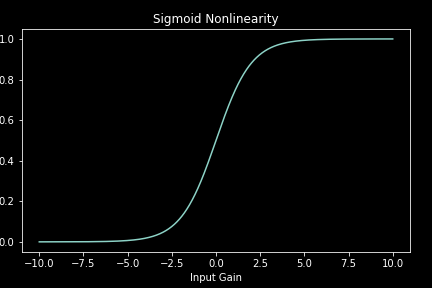
\includegraphics[height=2in]{../GatedRecurrentDistortion/Pics/sigmoid}
            \end{figure}
        \end{column}
        \begin{column}{0.5\linewidth}
            \begin{figure}
                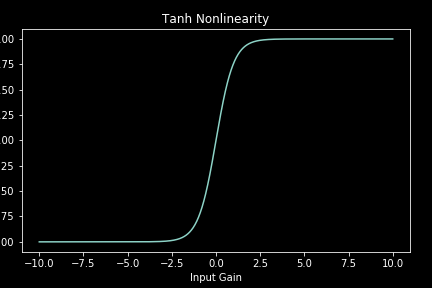
\includegraphics[height=2in]{../GatedRecurrentDistortion/Pics/tanh}
            \end{figure}
        \end{column}
    \end{columns}
\end{frame}

\begin{frame}{Gated Recurrent Distortion}
    \begin{figure}
        \centering
        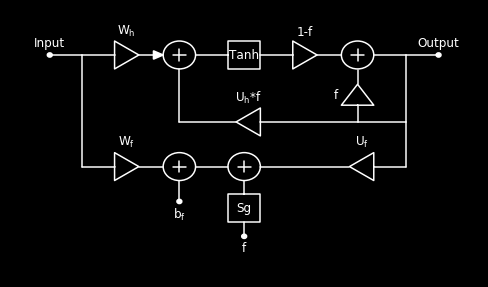
\includegraphics[height=2.5in]{../GatedRecurrentDistortion/Pics/gru_arch}
    \end{figure}
\end{frame}

\begin{frame}{Gated Recurrent Distortion: Parameters}
    \begin{figure}
        \centering
        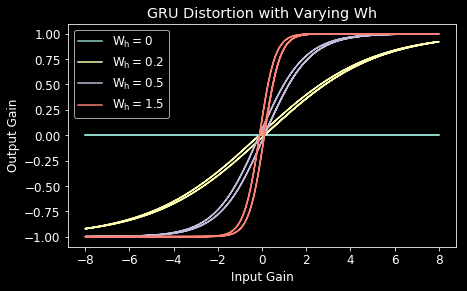
\includegraphics[height=2.5in]{../GatedRecurrentDistortion/Pics/wh}
    \end{figure}
\end{frame}

\begin{frame}{Gated Recurrent Distortion: Parameters}
    \begin{columns}
        \begin{column}{0.5\linewidth}
            \begin{figure}
                \centering
                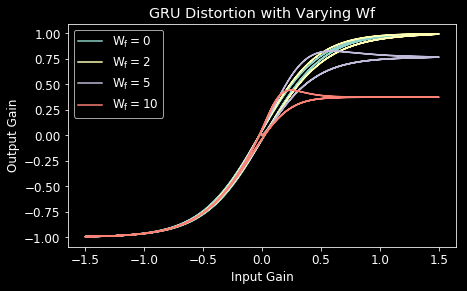
\includegraphics[width=2.75in]{../GatedRecurrentDistortion/Pics/wf}
            \end{figure}
        \end{column}
        \begin{column}{0.5\linewidth}
            \begin{figure}
                \centering
                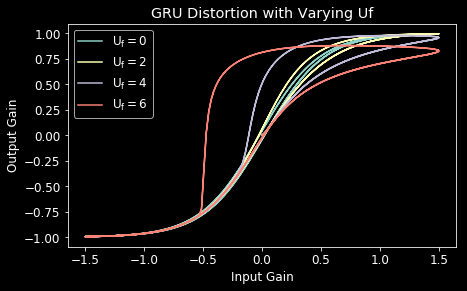
\includegraphics[width=2.75in]{../GatedRecurrentDistortion/Pics/uf}
            \end{figure}
        \end{column}
    \end{columns}
\end{frame}

\begin{frame}{Gated Recurrent Distortion: Parameters}
    \begin{columns}
        \begin{column}{0.5\linewidth}
            \begin{figure}
                \centering
                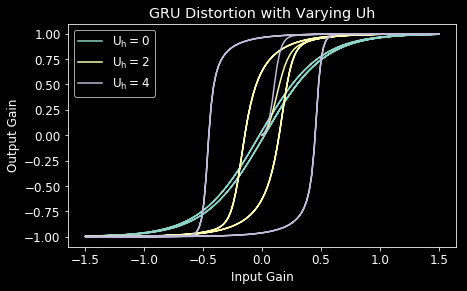
\includegraphics[width=2.75in]{../GatedRecurrentDistortion/Pics/uh}
            \end{figure}
        \end{column}
        \begin{column}{0.5\linewidth}
            \begin{figure}
                \centering
                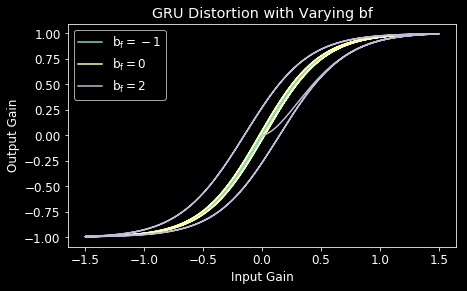
\includegraphics[width=2.75in]{../GatedRecurrentDistortion/Pics/bf}
            \end{figure}
        \end{column}
    \end{columns}
\end{frame}

\begin{frame}{Gated Recurrent Distortion: Harmonic Response}
    \begin{columns}
        \begin{column}{0.5\linewidth}
            \begin{figure}
                \centering
                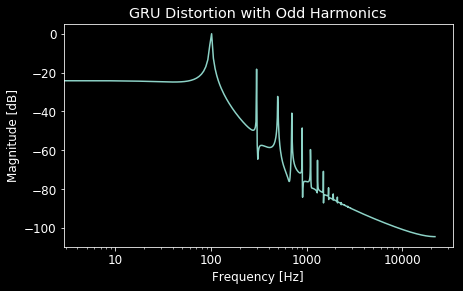
\includegraphics[width=2.75in]{../GatedRecurrentDistortion/Pics/odd_harm}
            \end{figure}
        \end{column}
        \begin{column}{0.5\linewidth}
            \begin{figure}
                \centering
                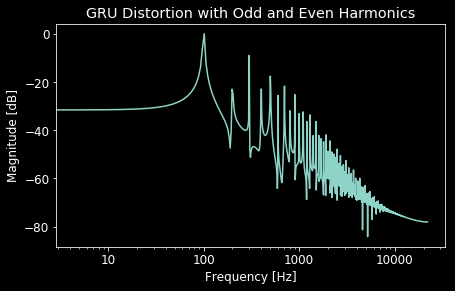
\includegraphics[width=2.75in]{../GatedRecurrentDistortion/Pics/all_harm}
            \end{figure}
        \end{column}
    \end{columns}
\end{frame}
